\documentclass{article}

\usepackage{tikz}

\begin{document}

\begin{minipage}{0.3\textwidth}
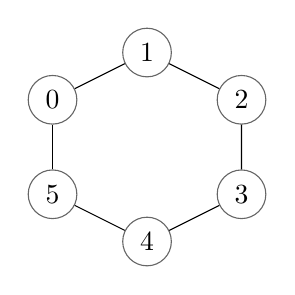
\begin{tikzpicture}
  [scale=.3,auto=left,every node/.style={circle, draw = black!60}]
  \node (n0) at (1,8) {0};
  \node (n1) at (5,10)  {1};
  \node (n2) at (9,8)  {2};
  \node (n5) at (1,4) {5};
  \node (n4) at (5,2)  {4};
  \node (n3) at (9,4)  {3};

  \foreach \from/\to in {n0/n1,n1/n2,n2/n3,n3/n4,n4/n5,n5/n0}
    \draw (\from) -- (\to);
\end{tikzpicture}
\end{minipage}
\hspace{1cm}
\begin{minipage}{0.3\textwidth}
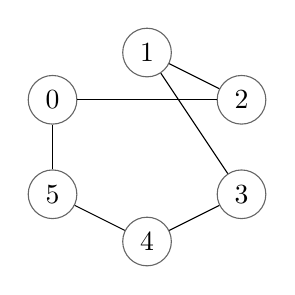
\begin{tikzpicture}
  [scale=.3,auto=left,every node/.style={circle, draw = black!60}]
  \node (n0) at (1,8) {0};
  \node (n1) at (5,10)  {1};
  \node (n2) at (9,8)  {2};
  \node (n5) at (1,4) {5};
  \node (n4) at (5,2)  {4};
  \node (n3) at (9,4)  {3};

  \foreach \from/\to in {n0/n2,n1/n2,n1/n3,n3/n4,n4/n5,n5/n0}
    \draw (\from) -- (\to);
\end{tikzpicture}
\end{minipage}
\hspace{1cm}
\begin{minipage}{0.3\textwidth}

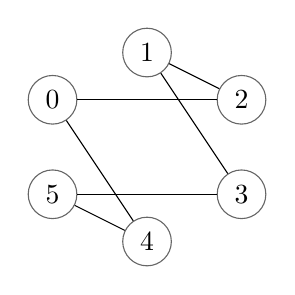
\begin{tikzpicture}
  [scale=.3,auto=left,every node/.style={circle, draw = black!60}]
  \node (n0) at (1,8) {0};
  \node (n1) at (5,10)  {1};
  \node (n2) at (9,8)  {2};
  \node (n5) at (1,4) {5};
  \node (n4) at (5,2)  {4};
  \node (n3) at (9,4)  {3};

  \foreach \from/\to in {n0/n2,n1/n2,n1/n3,n3/n5,n4/n5,n4/n0}
    \draw (\from) -- (\to);
\end{tikzpicture}
\end{minipage}

\vspace{2cm}

\begin{minipage}{0.3\textwidth}
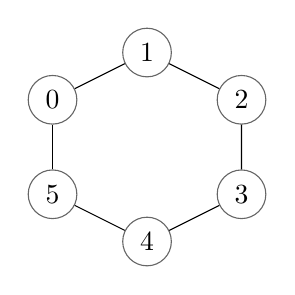
\begin{tikzpicture}
  [scale=.3,auto=left,every node/.style={circle, draw = black!60}]
  \node (n0) at (1,8) {0};
  \node (n1) at (5,10)  {1};
  \node (n2) at (9,8)  {2};
  \node (n5) at (1,4) {5};
  \node (n4) at (5,2)  {4};
  \node (n3) at (9,4)  {3};

  \foreach \from/\to in {n0/n1,n1/n2,n2/n3,n3/n4,n4/n5,n5/n0}
    \draw (\from) -- (\to);
\end{tikzpicture}
\end{minipage}
\hspace{1cm}
\begin{minipage}{0.3\textwidth}
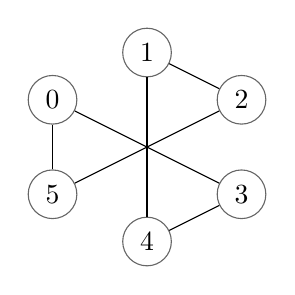
\begin{tikzpicture}
  [scale=.3,auto=left,every node/.style={circle, draw = black!60}]
  \node (n0) at (1,8) {0};
  \node (n1) at (5,10)  {1};
  \node (n2) at (9,8)  {2};
  \node (n5) at (1,4) {5};
  \node (n4) at (5,2)  {4};
  \node (n3) at (9,4)  {3};

  \foreach \from/\to in {n5/n2,n1/n2,n4/n3,n3/n0,n4/n1,n5/n0}
    \draw (\from) -- (\to);
\end{tikzpicture}
\end{minipage}

\end{document}